\documentclass{beamer}

\usetheme{default}
\usecolortheme{default}

% Remove navigation symbols
\setbeamertemplate{navigation symbols}{}

% White background
\setbeamercolor{background canvas}{bg=white}
\setbeamercolor{normal text}{fg=black}

% Remove frame titles
\setbeamertemplate{frametitle}{}

% Packages
\usepackage{tikz}
\usetikzlibrary{arrows.meta, positioning, calc, shapes.geometric, fit, backgrounds, patterns}
\usepackage{pgfplots}
\pgfplotsset{compat=1.18}
\usepackage{amsmath}
\usepackage{amssymb}
\usepackage{sfmath}

\begin{document}

\begin{frame}
  \centering
  \vspace{2cm}
  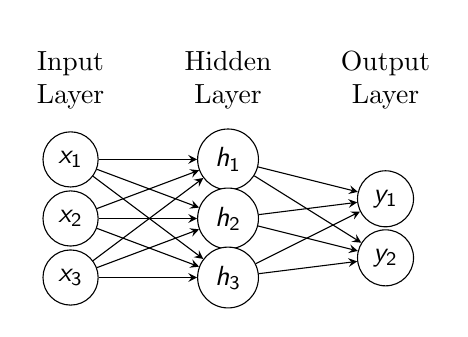
\begin{tikzpicture}[
    neuron/.style={circle, draw=black, fill=white, minimum size=16pt},
    arrow/.style={->, >=stealth}
  ]
    % Input layer
    \node[neuron] (i1) at (0,1.5) {$x_1$};
    \node[neuron] (i2) at (0,0.75) {$x_2$};
    \node[neuron] (i3) at (0,0) {$x_3$};
    
    % Hidden layer
    \node[neuron] (h1) at (2,1.5) {$h_1$};
    \node[neuron] (h2) at (2,0.75) {$h_2$};
    \node[neuron] (h3) at (2,0) {$h_3$};
    
    % Output layer
    \node[neuron] (o1) at (4,1) {$y_1$};
    \node[neuron] (o2) at (4,0.25) {$y_2$};
    
    % Connections
    \foreach \i in {1,2,3}
        \foreach \j in {1,2,3}
            \draw[arrow] (i\i) -- (h\j);
    
    \foreach \i in {1,2,3}
        \foreach \j in {1,2}
            \draw[arrow] (h\i) -- (o\j);
    
    % Labels
    \node[align=center] at (0,2.6) {\scriptsize \\Input\\Layer};
    \node[align=center] at (2,2.6) {\scriptsize \\Hidden\\Layer};
    \node[align=center] at (4,2.6) {\scriptsize \\Output\\Layer};
  \end{tikzpicture}
\end{frame}

\begin{frame}
  \centering
  \vspace{1cm}
  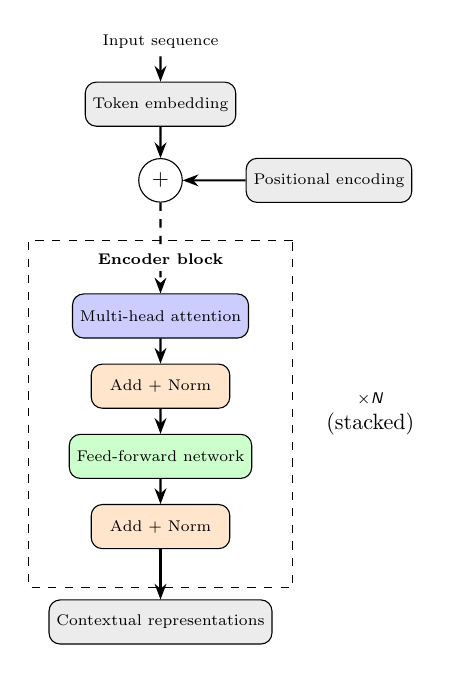
\begin{tikzpicture}[scale=0.8, every node/.style={transform shape},
    block/.style={draw, rounded corners, minimum width=2.2cm, minimum height=0.7cm, align=center},
    thinarrow/.style={-{Stealth[length=2mm,width=1.5mm]}, thick},
    node distance=4mm
  ]
    % Input tokens
    \node (tok) {\scriptsize Input sequence};
    % Token embedding
    \node[block, fill=gray!15, below=of tok] (emb) {\scriptsize Token embedding};
    % Plus
    \node[draw, circle, below=of emb, yshift=-1mm] (sum) {$+$};
    % Positional encoding
    \node[block, fill=gray!15, right=of sum, xshift=6mm] (posenc) {\scriptsize Positional encoding};

    % Arrows
    \draw[thinarrow] (tok) -- (emb);
    \draw[thinarrow] (emb) -- (sum);
    \draw[thinarrow] (posenc) -- (sum);

    % Encoder block
    \node[below=0.6cm of sum, draw, dashed, inner sep=6pt, minimum height=5.5cm, minimum width=4.2cm] (enc) {};
    
    % Inside encoder
    \node[block, fill=blue!20] at (enc.north) [yshift=-12mm] (mha) {\scriptsize Multi-head attention};
    \node[block, fill=orange!20, below=of mha] (add1) {\scriptsize Add + Norm};
    \node[block, fill=green!20, below=of add1] (ffn) {\scriptsize Feed-forward network};
    \node[block, fill=orange!20, below=of ffn] (add2) {\scriptsize Add + Norm};

    % Arrows
    \draw[thinarrow, dashed] (sum) -- (mha);
    \node[rectangle, fill=white, draw=none, inner sep=3pt] at ($(enc.north)-(0,3mm)$) {\scriptsize\textbf{Encoder block}};
    \draw[thinarrow] (mha) -- (add1);
    \draw[thinarrow] (add1) -- (ffn);
    \draw[thinarrow] (ffn) -- (add2);

    % Stack indication
    \node[right=of enc, align=center] (stack) {\scriptsize $\times N$\\(stacked)};

    % Output
    \node[block, fill=gray!15, below=8mm of add2] (out) {\scriptsize Contextual representations};
    \draw[thinarrow] (add2) -- (out);
  \end{tikzpicture}
\end{frame}

\begin{frame}
  \centering
  \vspace{3cm}
  \begin{minipage}{0.8\textwidth}
    \centering
    $$\pi(\cdot \, ; \, \theta_\pi) : (\mathbb{R}^l)^n \to \mathbb{R}^d$$
    
    \vspace{1.5cm}
    
    $$\psi(\mathbf{p} \, ; \, \theta_\psi) = \psi(\mathbf{p} \, ; \, \theta_\psi, \theta_\pi) = \pi(\Phi(\mathbf{p} \, ; \, \theta_\Phi) \, ; \, \theta_\pi) \in \mathbb{R}^d$$
  \end{minipage}
\end{frame}

\begin{frame}
    \centering
    % ----- Partition in feature space -----
    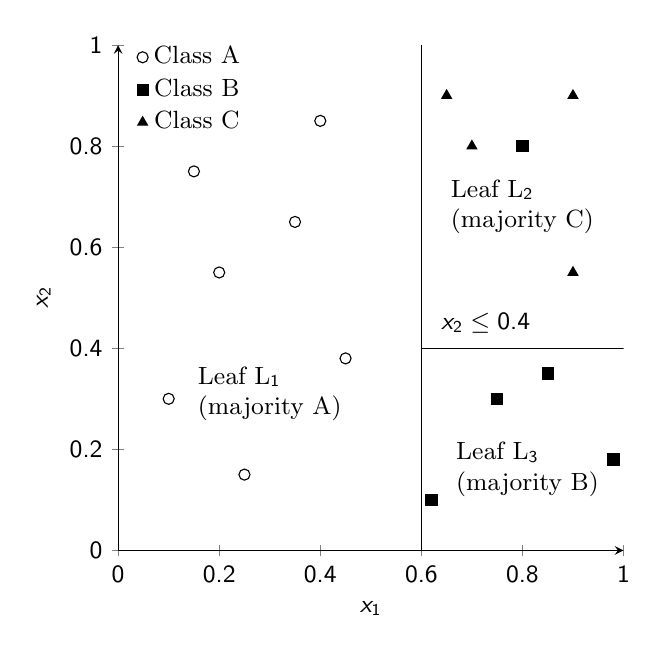
\begin{tikzpicture}
      \begin{axis}[
          width=8cm,height=8cm,
          xmin=0,xmax=1,ymin=0,ymax=1,
          xlabel={$x_1$},ylabel={$x_2$},
          axis x line=bottom, axis y line=left,
          xtick={0,0.2,0.4,0.6,0.8,1.0},
          ytick={0,0.2,0.4,0.6,0.8,1.0},
          tick label style={font=\small},
          label style={font=\small},
          legend style={draw=none,fill=none,at={(0.02,1.02)},anchor=north west,font=\small}
        ]
        % Class A (circles)
        \addplot[only marks,mark=o,mark size=2pt] coordinates {
          (0.15,0.75) (0.20,0.55) (0.35,0.65) (0.40,0.85) (0.10,0.30)
          (0.25,0.15) (0.45,0.38)
        };
        % Class B (squares)
        \addplot[only marks,mark=square*,mark size=2pt] coordinates {
          (0.80,0.80) (0.75,0.30) (0.98,0.18)
          (0.62,0.10) (0.85,0.35)
        };

        % Class C (triangles)
        \addplot[only marks,mark=triangle*,mark size=2pt] coordinates {
            (0.70,0.80) (0.90,0.55) (0.65, 0.90) (0.90,0.90)
        };

        \legend{Class A, Class B, Class C}
    
        % Split 1: x1 <= 0.6
        \addplot[domain=0:1, samples=2] ({0.6},{x});
        \node[font=\small,anchor=south] at (axis cs:0.55,1.1) {$x_1 \le 0.6$};
    
        % Split 2 (right child): x2 <= 0.4
        \addplot[domain=0.6:1, samples=2] ({x},{0.4});
        \node[font=\small,anchor=west] at (axis cs:0.62,0.45) {$x_2 \le 0.4$};
    
        % Region labels (leaves)
        \node[font=\small,align=left] at (axis cs:0.30,0.31) {Leaf L$_1$\\(majority A)};
        \node[font=\small,align=left] at (axis cs:0.80,0.68) {Leaf L$_2$\\(majority C)};
        \node[font=\small,align=left] at (axis cs:0.81,0.16) {Leaf L$_3$\\(majority B)};
      \end{axis}
    \end{tikzpicture}
\end{frame}

\begin{frame}
    \centering
    % ----- Corresponding binary tree -----
    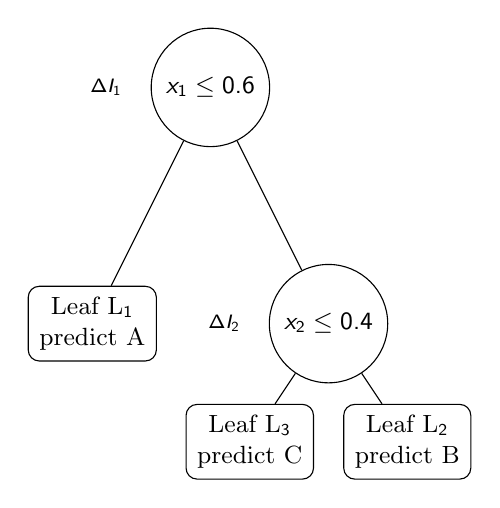
\begin{tikzpicture}[
        every node/.style={font=\small},
        leaf/.style={rectangle,draw,rounded corners,inner sep=4pt},
        split/.style={circle,draw,inner sep=4pt}
      ]
      % Root node
      \node[split] (root) at (0,2) {$x_1 \le 0.6$};
      
      % Left child (leaf)
      \node[leaf,align=center] (L1) at (-1.5,-1) {Leaf L$_1$ \\ predict A};
      \draw (root) -- (L1);
      
      % Right child (split node)
      \node[split] (r) at (1.5,-1) {$x_2 \le 0.4$};
      \draw (root) -- (r);
      
      % Right child's children (leaves)
      \node[leaf,align=center] (L3) at (0.5,-2.5) {Leaf L$_3$ \\ predict C};
      \node[leaf,align=center] (L2) at (2.5,-2.5) {Leaf L$_2$ \\ predict B};
      \draw (r) -- (L3);
      \draw (r) -- (L2);
      
      % impurity reductions (optional annotations)
      \node[font=\scriptsize,anchor=east] at ([xshift=-1.0cm]root) {$\Delta I_1$};
      \node[font=\scriptsize,anchor=east] at ([xshift=-1.0cm]r) {$\Delta I_2$};
    \end{tikzpicture}
\end{frame}

\begin{frame}
  \centering
  \vspace{0.5cm}
  \resizebox{!}{0.85\textheight}{
    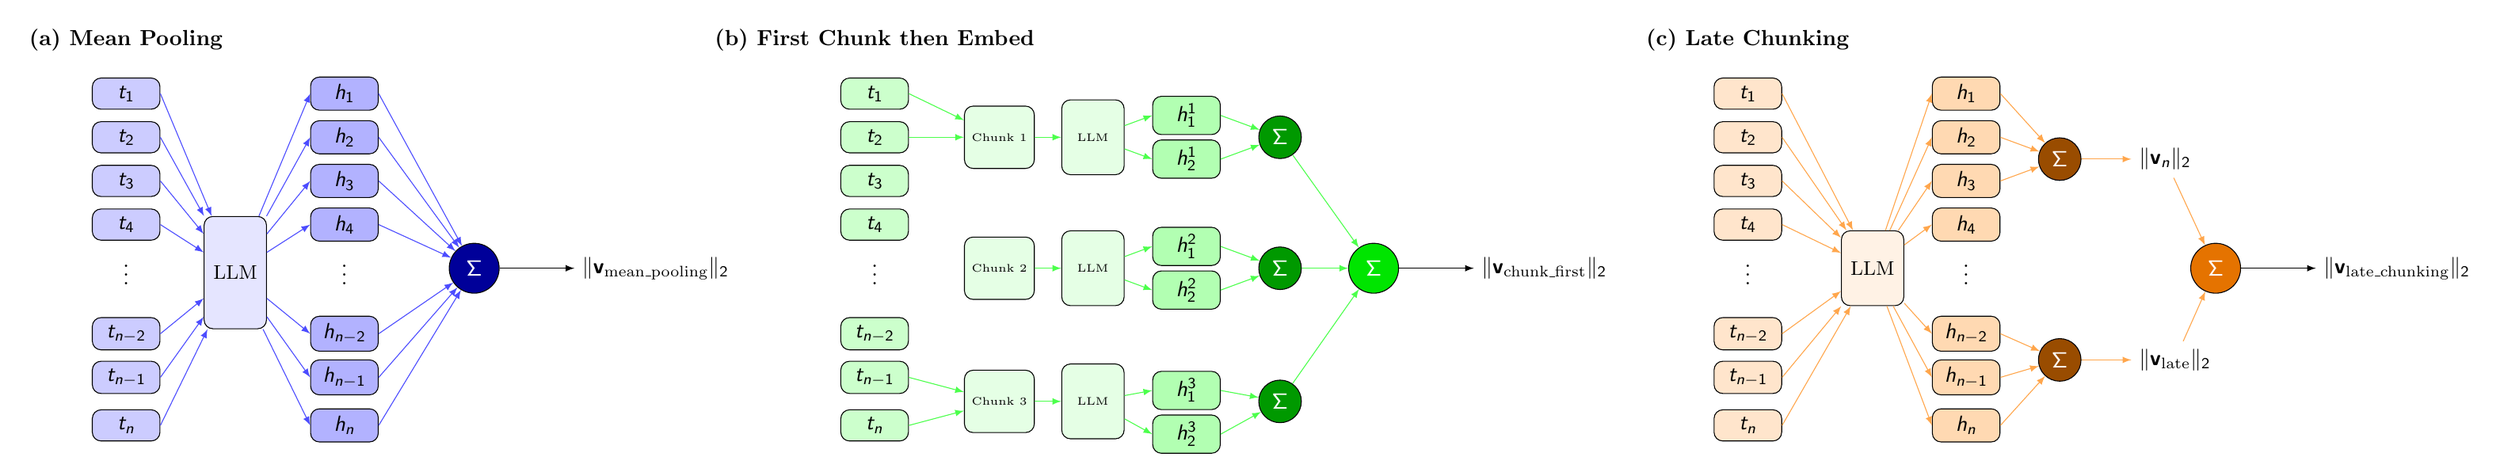
\begin{tikzpicture}[>=latex, node distance=0.8cm]

% -----------------------------------------------------
%  (a) MEAN POOLING
% -----------------------------------------------------
% Tokens at the top
\def\toptokens{4}
\foreach \i in {1,...,\toptokens}{
  \node[draw, fill=blue!20, rounded corners, minimum width=0.9cm, minimum height=0.5cm,
        align=center, text width=0.85cm] (ta\i) at (0,{-(\i-1)*0.7cm}) {$t_{\i}$};
}

% Ellipsis to indicate more tokens
\node[align=center] (ellipsis) at (0,{-(\toptokens)*0.7cm}) {$\vdots$};

% Tokens at the bottom (symmetrical: t_{n-2}, t_{n-1}, t_n) - more vertical spacing
\node[draw, fill=blue!20, rounded corners, minimum width=0.9cm, minimum height=0.5cm,
      align=center, text width=0.85cm] (tanm2) at (0,{-(\toptokens+1.5)*0.7cm}) {$t_{n-2}$};
\node[draw, fill=blue!20, rounded corners, minimum width=0.9cm, minimum height=0.5cm,
      align=center, text width=0.85cm] (tanm1) at (0,{-(\toptokens+2.5)*0.7cm}) {$t_{n-1}$};
\node[draw, fill=blue!20, rounded corners, minimum width=0.9cm, minimum height=0.5cm,
      align=center, text width=0.85cm] (tan) at (0,{-(\toptokens+3.6)*0.7cm}) {$t_n$};

% LLM box in the middle (taller and centered vertically between tokens and hidden states)
% Center it between top token and bottom token (moved higher)
\pgfmathsetmacro{\llmcenterY}{-(\toptokens+0.1)*0.7}
\node[draw, fill=blue!10, rounded corners, minimum width=1.0cm, minimum height=1.8cm,
      align=center] (llmA) at (1.75cm,\llmcenterY cm) {\small LLM};

% Hidden states parallel to tokens (further from LLM)
\foreach \i in {1,...,\toptokens}{
  \node[draw, fill=blue!30, rounded corners, minimum width=0.9cm, minimum height=0.5cm,
        align=center, text width=0.85cm] (ha\i) at (3.5cm,{-(\i-1)*0.7cm}) {$h_{\i}$};
}

% Ellipsis for hidden states
\node[align=center] (ellipsisH) at (3.5cm,{-(\toptokens)*0.7cm}) {$\vdots$};

% Hidden states at the bottom (matching token spacing)
\node[draw, fill=blue!30, rounded corners, minimum width=0.9cm, minimum height=0.5cm,
      align=center, text width=0.85cm] (hanm2) at (3.5cm,{-(\toptokens+1.5)*0.7cm}) {$h_{n-2}$};
\node[draw, fill=blue!30, rounded corners, minimum width=0.9cm, minimum height=0.5cm,
      align=center, text width=0.85cm] (hanm1) at (3.5cm,{-(\toptokens+2.5)*0.7cm}) {$h_{n-1}$};
\node[draw, fill=blue!30, rounded corners, minimum width=0.9cm, minimum height=0.5cm,
      align=center, text width=0.85cm] (han) at (3.5cm,{-(\toptokens+3.6)*0.7cm}) {$h_n$};

% Mean pooling symbol after hidden states
\node[circle, draw, fill=blue!60!black, text=white, minimum size=0.8cm,
      right=1.5cm of ellipsisH] (meanA) {$\Sigma$};

% Arrows from tokens to LLM (exit from right side of tokens)
\foreach \i in {1,...,\toptokens}{
  \draw[->, blue!70] (ta\i.east) -- (llmA);
}
\draw[->, blue!70] (tanm2.east) -- (llmA);
\draw[->, blue!70] (tanm1.east) -- (llmA);
\draw[->, blue!70] (tan.east) -- (llmA);

% Arrows from LLM to hidden states (enter from left side of hidden states)
\foreach \i in {1,...,\toptokens}{
  \draw[->, blue!70] (llmA) -- (ha\i.west);
}
\draw[->, blue!70] (llmA) -- (hanm2.west);
\draw[->, blue!70] (llmA) -- (hanm1.west);
\draw[->, blue!70] (llmA) -- (han.west);

% Arrows from hidden states to mean (exit from right side of hidden states)
\foreach \i in {1,...,\toptokens}{
  \draw[->, blue!70] (ha\i.east) -- (meanA);
}
\draw[->, blue!70] (hanm2.east) -- (meanA);
\draw[->, blue!70] (hanm1.east) -- (meanA);
\draw[->, blue!70] (han.east) -- (meanA);

% Output on the right (with L2 norm)
\node[right=1.2cm of meanA] (outA) {$\|\mathbf{v}_{\text{mean\_pooling}}\|_2$};
\draw[->] (meanA) -- (outA);

% Title
\node[above=0.3cm of ta1, anchor=south] {\textbf{(a) Mean Pooling}};

% -----------------------------------------------------
%  (b) FIRST CHUNK THEN EMBED
% -----------------------------------------------------
% X offset for second subplot (much further from first)
\def\xoffsetB{12cm}

% Tokens at the top
\foreach \i in {1,...,\toptokens}{
  \node[draw, fill=green!20, rounded corners, minimum width=0.9cm, minimum height=0.5cm,
        align=center, text width=0.85cm] (tb\i) at (\xoffsetB,{-(\i-1)*0.7cm}) {$t_{\i}$};
}

% Ellipsis to indicate more tokens
\node[align=center] (ellipsisB) at (\xoffsetB,{-(\toptokens)*0.7cm}) {$\vdots$};

% Tokens at the bottom (symmetrical: t_{n-2}, t_{n-1}, t_n) - matching spacing
\node[draw, fill=green!20, rounded corners, minimum width=0.9cm, minimum height=0.5cm,
      align=center, text width=0.85cm] (tbnm2) at (\xoffsetB,{-(\toptokens+1.5)*0.7cm}) {$t_{n-2}$};
\node[draw, fill=green!20, rounded corners, minimum width=0.9cm, minimum height=0.5cm,
      align=center, text width=0.85cm] (tbnm1) at (\xoffsetB,{-(\toptokens+2.5)*0.7cm}) {$t_{n-1}$};
\node[draw, fill=green!20, rounded corners, minimum width=0.9cm, minimum height=0.5cm,
      align=center, text width=0.85cm] (tbn) at (\xoffsetB,{-(\toptokens+3.6)*0.7cm}) {$t_n$};

% Chunking: Show 3 chunks (simplified representation)
% Chunk 1: tokens t1-t2
\node[draw, fill=green!10, rounded corners, minimum width=1.0cm, minimum height=1.0cm,
      align=center] (chunk1) at ($(\xoffsetB+2.0cm,{-1*0.7cm})$) {\tiny Chunk 1};
% Chunk 2: middle tokens
\node[draw, fill=green!10, rounded corners, minimum width=1.0cm, minimum height=1.0cm,
      align=center] (chunk2) at ($(\xoffsetB+2.0cm,{-(\toptokens)*0.7cm})$) {\tiny Chunk 2};
% Chunk 3: tokens t_{n-1}-t_n
\node[draw, fill=green!10, rounded corners, minimum width=1.0cm, minimum height=1.0cm,
      align=center] (chunk3) at ($(\xoffsetB+2.0cm,{-(\toptokens+3.05)*0.7cm})$) {\tiny Chunk 3};

% LLMs for each chunk
\node[draw, fill=green!10, rounded corners, minimum width=1.0cm, minimum height=1.2cm,
      align=center] (llmB1) at ($(\xoffsetB+3.5cm,{-1*0.7cm})$) {\tiny LLM};
\node[draw, fill=green!10, rounded corners, minimum width=1.0cm, minimum height=1.2cm,
      align=center] (llmB2) at ($(\xoffsetB+3.5cm,{-(\toptokens)*0.7cm})$) {\tiny LLM};
\node[draw, fill=green!10, rounded corners, minimum width=1.0cm, minimum height=1.2cm,
      align=center] (llmB3) at ($(\xoffsetB+3.5cm,{-(\toptokens+3.05)*0.7cm})$) {\tiny LLM};

% Hidden states per chunk (simplified - show a few)
\node[draw, fill=green!30, rounded corners, minimum width=0.9cm, minimum height=0.5cm,
      align=center, text width=0.85cm] (hb1) at ($(\xoffsetB+5.0cm,{-0.5*0.7cm})$) {$h_1^1$};
\node[draw, fill=green!30, rounded corners, minimum width=0.9cm, minimum height=0.5cm,
      align=center, text width=0.85cm] (hb2) at ($(\xoffsetB+5.0cm,{-1.5*0.7cm})$) {$h_2^1$};

\node[draw, fill=green!30, rounded corners, minimum width=0.9cm, minimum height=0.5cm,
      align=center, text width=0.85cm] (hb3) at ($(\xoffsetB+5.0cm,{-(\toptokens-0.5)*0.7cm})$) {$h_1^2$};
\node[draw, fill=green!30, rounded corners, minimum width=0.9cm, minimum height=0.5cm,
      align=center, text width=0.85cm] (hb4) at ($(\xoffsetB+5.0cm,{-(\toptokens+0.5)*0.7cm})$) {$h_2^2$};

\node[draw, fill=green!30, rounded corners, minimum width=0.9cm, minimum height=0.5cm,
      align=center, text width=0.85cm] (hb5) at ($(\xoffsetB+5.0cm,{-(\toptokens+2.8)*0.7cm})$) {$h_1^3$};
\node[draw, fill=green!30, rounded corners, minimum width=0.9cm, minimum height=0.5cm,
      align=center, text width=0.85cm] (hb6) at ($(\xoffsetB+5.0cm,{-(\toptokens+3.8)*0.7cm})$) {$h_2^3$};

% Pooling per chunk
\node[circle, draw, fill=green!60!black, text=white, minimum size=0.6cm] (poolB1) at ($(\xoffsetB+6.5cm,{-1*0.7cm})$) {$\Sigma$};
\node[circle, draw, fill=green!60!black, text=white, minimum size=0.6cm] (poolB2) at ($(\xoffsetB+6.5cm,{-(\toptokens)*0.7cm})$) {$\Sigma$};
\node[circle, draw, fill=green!60!black, text=white, minimum size=0.6cm] (poolB3) at ($(\xoffsetB+6.5cm,{-(\toptokens+3.05)*0.7cm})$) {$\Sigma$};

% Final aggregation (moved to the right of pooling nodes)
\node[circle, draw, fill=green!90!black, text=white, minimum size=0.8cm] (aggB) at ($(\xoffsetB+8.0cm,{-(\toptokens)*0.7cm})$) {$\Sigma$};

% Output (with L2 norm)
\node[right=1.2cm of aggB] (outB) {$\|\mathbf{v}_{\text{chunk\_first}}\|_2$};

% Arrows: tokens to chunks
\draw[->, green!70] (tb1.east) -- (chunk1);
\draw[->, green!70] (tb2.east) -- (chunk1);
% Removed arrow from ellipsisB to chunk2
\draw[->, green!70] (tbnm1.east) -- (chunk3);
\draw[->, green!70] (tbn.east) -- (chunk3);

% Arrows: chunks to LLMs
\draw[->, green!70] (chunk1) -- (llmB1);
\draw[->, green!70] (chunk2) -- (llmB2);
\draw[->, green!70] (chunk3) -- (llmB3);

% Arrows: LLMs to hidden states
\draw[->, green!70] (llmB1) -- (hb1.west);
\draw[->, green!70] (llmB1) -- (hb2.west);
\draw[->, green!70] (llmB2) -- (hb3.west);
\draw[->, green!70] (llmB2) -- (hb4.west);
\draw[->, green!70] (llmB3) -- (hb5.west);
\draw[->, green!70] (llmB3) -- (hb6.west);

% Arrows: hidden states to pooling
\draw[->, green!70] (hb1.east) -- (poolB1);
\draw[->, green!70] (hb2.east) -- (poolB1);
\draw[->, green!70] (hb3.east) -- (poolB2);
\draw[->, green!70] (hb4.east) -- (poolB2);
\draw[->, green!70] (hb5.east) -- (poolB3);
\draw[->, green!70] (hb6.east) -- (poolB3);

% Arrows: pooling to final aggregation
\draw[->, green!70] (poolB1) -- (aggB);
\draw[->, green!70] (poolB2) -- (aggB);
\draw[->, green!70] (poolB3) -- (aggB);

% Arrow: aggregation to output
\draw[->] (aggB) -- (outB);

% Title
\node[above=0.3cm of tb1, anchor=south] {\textbf{(b) First Chunk then Embed}};

% -----------------------------------------------------
%  (c) LATE CHUNKING
% -----------------------------------------------------
% X offset for third subplot (much further from second)
\def\xoffsetC{26cm}

% Tokens at the top
\foreach \i in {1,...,\toptokens}{
  \node[draw, fill=orange!20, rounded corners, minimum width=0.9cm, minimum height=0.5cm,
        align=center, text width=0.85cm] (tc\i) at (\xoffsetC,{-(\i-1)*0.7cm}) {$t_{\i}$};
}

% Ellipsis to indicate more tokens
\node[align=center] (ellipsisC) at (\xoffsetC,{-(\toptokens)*0.7cm}) {$\vdots$};

% Tokens at the bottom (symmetrical: t_{n-2}, t_{n-1}, t_n) - matching spacing
\node[draw, fill=orange!20, rounded corners, minimum width=0.9cm, minimum height=0.5cm,
      align=center, text width=0.85cm] (tcnm2) at (\xoffsetC,{-(\toptokens+1.5)*0.7cm}) {$t_{n-2}$};
\node[draw, fill=orange!20, rounded corners, minimum width=0.9cm, minimum height=0.5cm,
      align=center, text width=0.85cm] (tcnm1) at (\xoffsetC,{-(\toptokens+2.5)*0.7cm}) {$t_{n-1}$};
\node[draw, fill=orange!20, rounded corners, minimum width=0.9cm, minimum height=0.5cm,
      align=center, text width=0.85cm] (tcn) at (\xoffsetC,{-(\toptokens+3.6)*0.7cm}) {$t_n$};

% LLM box (single LLM like mean pooling)
\node[draw, fill=orange!10, rounded corners, minimum width=1.0cm, minimum height=1.2cm,
      align=center] (llmC) at ($(\xoffsetC+2.0cm,{-(\toptokens)*0.7cm})$) {\small LLM};

% Hidden states parallel to tokens (like mean pooling)
\foreach \i in {1,...,\toptokens}{
  \node[draw, fill=orange!30, rounded corners, minimum width=0.9cm, minimum height=0.5cm,
        align=center, text width=0.85cm] (hc\i) at ($(\xoffsetC+3.5cm,{-(\i-1)*0.7cm})$) {$h_{\i}$};
}

% Ellipsis for hidden states
\node[align=center] (ellipsisHC) at ($(\xoffsetC+3.5cm,{-(\toptokens)*0.7cm})$) {$\vdots$};

% Hidden states at the bottom (matching token spacing)
\node[draw, fill=orange!30, rounded corners, minimum width=0.9cm, minimum height=0.5cm,
      align=center, text width=0.85cm] (hcnm2) at ($(\xoffsetC+3.5cm,{-(\toptokens+1.5)*0.7cm})$) {$h_{n-2}$};
\node[draw, fill=orange!30, rounded corners, minimum width=0.9cm, minimum height=0.5cm,
      align=center, text width=0.85cm] (hcnm1) at ($(\xoffsetC+3.5cm,{-(\toptokens+2.5)*0.7cm})$) {$h_{n-1}$};
\node[draw, fill=orange!30, rounded corners, minimum width=0.9cm, minimum height=0.5cm,
      align=center, text width=0.85cm] (hcn) at ($(\xoffsetC+3.5cm,{-(\toptokens+3.6)*0.7cm})$) {$h_n$};

% Windowed pooling: Show 2 windows (overlapping)
% Window 1: top hidden states
\node[circle, draw, fill=orange!60!black, text=white, minimum size=0.6cm] (poolC1) at ($(\xoffsetC+5.0cm,{-1.5*0.7cm})$) {$\Sigma$};
% Window 2: bottom hidden states  
\node[circle, draw, fill=orange!60!black, text=white, minimum size=0.6cm] (poolC2) at ($(\xoffsetC+5.0cm,{-(\toptokens+2.1)*0.7cm})$) {$\Sigma$};

% Window vectors with L2 norm notation
\node[right=0.8cm of poolC1] (vecC1) {$\|\mathbf{v}_n\|_2$};
\node[right=0.8cm of poolC2] (vecC2) {$\|\mathbf{v}_{\text{late}}\|_2$};

% Final aggregation (moved to the right of window vectors)
\node[circle, draw, fill=orange!90!black, text=white, minimum size=0.8cm] (aggC) at ($(\xoffsetC+7.5cm,{-(\toptokens)*0.7cm})$) {$\Sigma$};

% Output (with L2 norm)
\node[right=1.2cm of aggC] (outC) {$\|\mathbf{v}_{\text{late\_chunking}}\|_2$};

% Arrows from tokens to LLM (exit from right side)
\foreach \i in {1,...,\toptokens}{
  \draw[->, orange!70] (tc\i.east) -- (llmC);
}
\draw[->, orange!70] (tcnm2.east) -- (llmC);
\draw[->, orange!70] (tcnm1.east) -- (llmC);
\draw[->, orange!70] (tcn.east) -- (llmC);

% Arrows from LLM to hidden states (enter from left side)
\foreach \i in {1,...,\toptokens}{
  \draw[->, orange!70] (llmC) -- (hc\i.west);
}
\draw[->, orange!70] (llmC) -- (hcnm2.west);
\draw[->, orange!70] (llmC) -- (hcnm1.west);
\draw[->, orange!70] (llmC) -- (hcn.west);

% Arrows from hidden states to windowed pooling (exit from right side)
% Window 1: connects to top hidden states
\draw[->, orange!70] (hc1.east) -- (poolC1);
\draw[->, orange!70] (hc2.east) -- (poolC1);
\draw[->, orange!70] (hc3.east) -- (poolC1);
% Window 2: connects to bottom hidden states
\draw[->, orange!70] (hcnm2.east) -- (poolC2);
\draw[->, orange!70] (hcnm1.east) -- (poolC2);
\draw[->, orange!70] (hcn.east) -- (poolC2);

% Arrows from pooling to window vectors
\draw[->, orange!70] (poolC1) -- (vecC1);
\draw[->, orange!70] (poolC2) -- (vecC2);

% Arrows from window vectors to final aggregation
\draw[->, orange!70] (vecC1) -- (aggC);
\draw[->, orange!70] (vecC2) -- (aggC);

% Arrow: aggregation to output
\draw[->] (aggC) -- (outC);

% Title
\node[above=0.3cm of tc1, anchor=south] {\textbf{(c) Late Chunking}};

    \end{tikzpicture}
  }
\end{frame}

\begin{frame}
  \centering
  \vspace{2cm}
  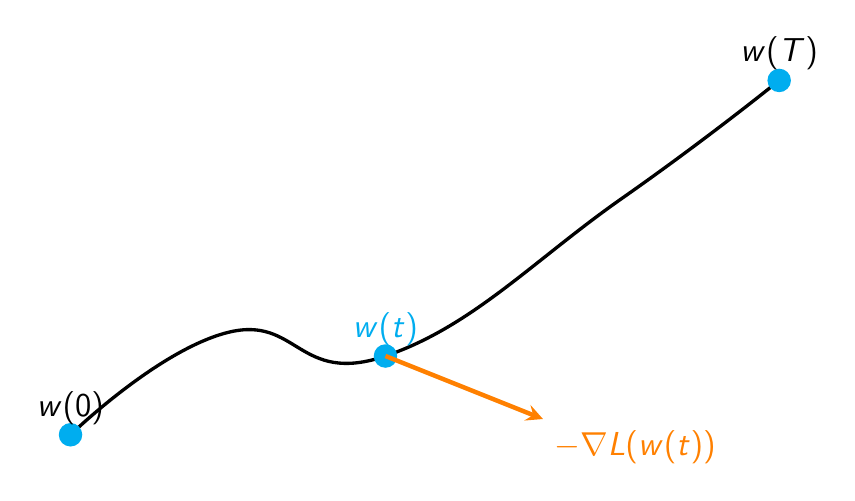
\begin{tikzpicture}[>=stealth, thick,
      point/.style={circle, fill=cyan, inner sep=3pt},
      vector/.style={->, orange, ultra thick},
      label_text/.style={font=\sffamily\large}
  ]

  % Define coordinates for the trajectory
  \coordinate (w0) at (0, 1.5);
  \coordinate (wt) at (4, 2.5);
  \coordinate (wT) at (9, 6);

  % Draw the curved trajectory
  \draw[black, very thick] plot [smooth, tension=0.8] coordinates {(w0) (2, 2.8) (wt) (7, 4.5) (wT)};

  % Draw the points
  \node[point] at (w0) {};
  \node[point] at (wt) {};
  \node[point] at (wT) {};

  % Draw and label the negative gradient vector at w(t)
  \draw[vector] (wt) -- ++(2, -0.8) node[below right, orange, label_text] {$-\nabla L(w(t))$};

  % Label the points
  \node[above, label_text] at (w0) {$w(0)$};
  \node[above, label_text, cyan] at (wt) {$w(t)$};
  \node[above, label_text] at (wT) {$w(T)$};

  \end{tikzpicture}
\end{frame}

\begin{frame}
  \centering
  \vspace{0.3cm}
  \resizebox{!}{0.9\textheight}{
    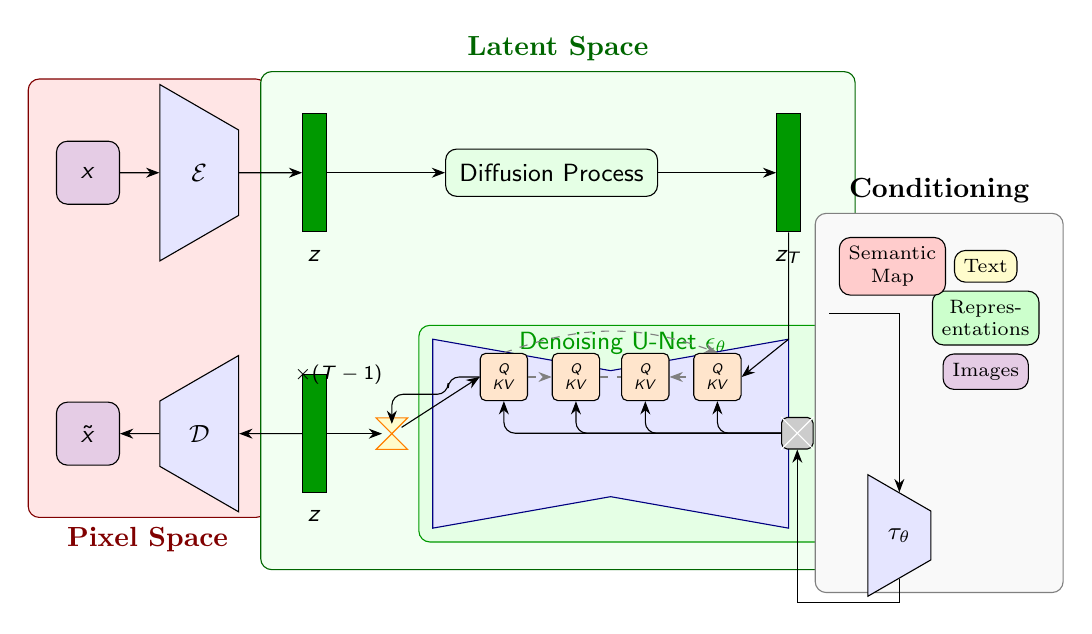
\begin{tikzpicture}[
        font=\sffamily\small,
        >=Stealth,
        node distance=1cm and 1cm,
        % Styles
        pixel_node/.style={draw, rectangle, rounded corners, fill=violet!20, minimum size=0.8cm, inner sep=2pt},
        trap_enc/.style={draw, trapezium, trapezium angle=60, shape border rotate=270, fill=blue!10, minimum height=1cm, inner sep=0pt},
        trap_dec/.style={draw, trapezium, trapezium angle=60, shape border rotate=90, fill=blue!10, minimum height=1cm, inner sep=0pt},
        latent_vec/.style={draw, rectangle, fill=green!60!black, minimum height=1.5cm, minimum width=0.3cm},
        process_box/.style={draw, rectangle, rounded corners, fill=green!10, minimum height=0.6cm, inner sep=5pt},
        qkv_box/.style={draw, rectangle, fill=orange!20, rounded corners=2pt, minimum width=0.6cm, minimum height=0.6cm, font=\scriptsize},
        cond_enc/.style={draw, trapezium, trapezium angle=60, shape border rotate=270, fill=blue!10, minimum height=0.8cm},
        switch/.style={draw, rectangle, fill=black!20, minimum size=0.4cm},
        label_text/.style={font=\bfseries}
    ]

    % --- 1. Pixel Space (Left) ---
    \node[pixel_node] (x) {$x$};
    \node[trap_enc, right=0.5cm of x] (E) {$\mathcal{E}$};
    \node[latent_vec, right=0.8cm of E] (z) {};
    \node[below=0.1cm of z] {$z$};

    \node[pixel_node, below=2.5cm of x] (x_tilde) {$\tilde{x}$};
    \node[trap_dec, right=0.5cm of x_tilde] (D) {$\mathcal{D}$};
    % Re-use vertical alignment from z for the lower latent vector
    \node[latent_vec] (z_bottom) at (z |- D) {};
    \node[below=0.1cm of z_bottom] {$z$};

    % Connections Pixel Space
    \draw[->] (x) -- (E);
    \draw[->] (E) -- (z);
    \draw[->] (z_bottom) -- (D);
    \draw[->] (D) -- (x_tilde);

    % --- 2. Latent Space (Center Top) ---
    \node[process_box, right=1.5cm of z] (diff_proc) {Diffusion Process};
    \node[latent_vec, right=1.5cm of diff_proc] (zT) {};
    \node[below=0.1cm of zT] {$z_T$};

    \draw[->] (z) -- (diff_proc);
    \draw[->] (diff_proc) -- (zT);

    % --- 3. Denoising U-Net (Center Bottom) ---
    % We construct the visual representation of the U-Net manually to match the diagram
    % Coordinate definitions for the U-Net container
    \coordinate (unet_tl) at ($(z_bottom)+(1.5, 1.2)$);
    \coordinate (unet_bl) at ($(z_bottom)+(1.5, -1.2)$);
    \coordinate (unet_tr) at ($(zT |- unet_tl)$);
    \coordinate (unet_br) at ($(zT |- unet_bl)$);
    \coordinate (unet_mid_t) at ($(unet_tl)!0.5!(unet_tr) + (0, -0.4)$);
    \coordinate (unet_mid_b) at ($(unet_bl)!0.5!(unet_br) + (0, 0.4)$);

    % Draw U-Net Background Shape
    \filldraw[draw=blue!50!black, fill=blue!10] 
        (unet_tl) -- (unet_mid_t) -- (unet_tr) -- (unet_br) -- (unet_mid_b) -- (unet_bl) -- cycle;

    % Internal QKV Blocks
    \node[qkv_box] (qkv1) at ($(unet_tl)!0.2!(unet_br)$) {$Q \atop K V$};
    \node[qkv_box, right=0.3cm of qkv1] (qkv2) {$Q \atop K V$};
    \node[qkv_box] (qkv4) at ($(unet_tr)!0.2!(unet_bl)$) {$Q \atop K V$};
    \node[qkv_box, left=0.3cm of qkv4] (qkv3) {$Q \atop K V$};

    % Denoising Step (Bowtie symbol)
    \node[right=0.5cm of z_bottom] (bowtie_center) {};
    \draw[fill=yellow!20, draw=orange] ($(bowtie_center)+(0,0.2)$) -- ($(bowtie_center)+(0.4,0.2)$) -- ($(bowtie_center)+(0,-0.2)$) -- ($(bowtie_center)+(0.4,-0.2)$) -- cycle;
    \node (denoise_step) at ($(bowtie_center)+(0.2,0)$) {};

    % Switch symbol (concatenation/injection point)
    \node[switch, below right=0.2cm and 0.5cm of qkv4, rounded corners=2pt] (switch_node) {};
    \draw[white] (switch_node.south west) -- (switch_node.north east);
    \draw[white] (switch_node.north west) -- (switch_node.south east);

    % Connections Latent Space Bottom
    \draw[->] (zT) -- (zT |- unet_tr) -- (qkv4.east); % Input from Noisy Latent
    \draw[->] (z_bottom) -- (denoise_step); 
    \draw[->] (denoise_step) -- (qkv1.west);
    \draw[dashed, gray, ->] (qkv1) -- (qkv2);
    \draw[dashed, gray] (qkv2) -- (qkv3);
    \draw[dashed, gray, <-] (qkv3) -- (qkv4);

    % U-Net Skip Connection (conceptual)
    \draw[dashed, gray, ->, bend left=20] (qkv1.north) to (qkv4.north);

    % Cycle z_T-1 loop
    \draw[->, rounded corners] (qkv1.west) -- ++(-0.4,0) |- ($(denoise_step)+(0,0.5)$) -- (denoise_step.north);
    \node[font=\scriptsize, above left] at ($(denoise_step)+(0,0.5)$) {$\times(T-1)$};

    % --- 4. Conditioning (Right) ---
    \node[cond_enc, right=1.0cm of unet_br, anchor=south west, yshift=-0.5cm] (tau) {$\tau_\theta$};

    % Conditioning Inputs
    \node[draw, rounded corners, fill=violet!20, align=center, font=\scriptsize, above right=1.5cm and 0.2cm of tau] (c_img) {Images};
    \node[draw, rounded corners, fill=green!20, align=center, font=\scriptsize, above=0.1cm of c_img] (c_rep) {Repres-\\entations};
    \node[draw, rounded corners, fill=yellow!20, align=center, font=\scriptsize, above=0.1cm of c_rep] (c_txt) {Text};
    \node[draw, rounded corners, fill=red!20, align=center, font=\scriptsize, left=0.1cm of c_txt] (c_map) {Semantic\\Map};

    % Grouping Conditioning
    \node[fit=(c_img)(c_rep)(c_txt)(c_map)](cond_group){};

    % Connections Conditioning
    \draw[->] (cond_group) -| (tau.north);
    \draw[->] (tau.south) -- ++(0,-0.3) -| (switch_node.south);

    % Inject Conditioning into QKV
    \foreach \x in {qkv1, qkv2, qkv3, qkv4}
        \draw[->, rounded corners] (switch_node.west) -| (\x.south);

    % --- 5. Backgrounds & Labels ---

    % Pixel Space Background (Red)
    \begin{scope}[on background layer]
        \node[fit=(x)(x_tilde)(E)(D), draw=red!50!black, fill=red!10, rounded corners, inner sep=10pt, label={[red!50!black, font=\bfseries]south:Pixel Space}] (pixel_bg) {};
    \end{scope}

    % Latent Space Background (Green)
    \begin{scope}[on background layer]
        \node[fit=(z)(zT)(unet_tl)(unet_br)(qkv1)(switch_node), draw=green!40!black, fill=green!5, rounded corners, inner sep=15pt, label={[green!40!black, font=\bfseries]north:Latent Space}] (latent_bg) {};
        % Inner U-Net Box
        \node[fit=(unet_tl)(unet_br)(switch_node), draw=green!60!black, fill=green!10, rounded corners, inner sep=5pt, label={[green!60!black, yshift=-0.5cm]north:Denoising U-Net $\epsilon_\theta$}] {};
    \end{scope}

    % Conditioning Background (Gray)
    \begin{scope}[on background layer]
        \node[fit=(cond_group)(tau), draw=gray, fill=gray!5, rounded corners, inner sep=5pt, label={[black, font=\bfseries]north:Conditioning}] (cond_bg) {};
    \end{scope}

    % Legend
    \node[below=1cm of pixel_bg.south west, anchor=west] (leg1) {};
    % (Legend items can be added here similar to the original image if required)

    \end{tikzpicture}
  }
\end{frame}

\end{document}
